\chapter{Arduino-Programmcode für die Mischmaschine}\label{Anhang_A}
\lstinputlisting[language=c++, style=algoBericht, basicstyle=\tiny\sffamily, captionpos=b, caption={Arduino-Programmcode für die Mischmaschine}, escapeinside={//*}{*)}]{./Listings/GetraenkemischmaschineV2.ino}

\chapter{Spracherkennung auf dem Raspberry Pi}\label{Anhang_B}
\lstinputlisting[language=python, style=algoBericht, basicstyle=\tiny\sffamily, captionpos=b, caption={Spracherkennung auf dem Raspberry Pi}, escapeinside={\#*}{*)}]{./Listings/main.py}
Es sei darauf hingewiesen, dass die C-Funktion, die in den Zeilen acht bis elf definiert wird, lediglich dem Verstecken unerwünschter Meldungen von der \textit{libasound}-Bibliothek dient.

\chapter{Sprachverarbeitung auf dem Raspberry Pi}\label{Anhang_C}
\lstinputlisting[language=python, style=algoBericht, basicstyle=\tiny\sffamily, captionpos=b, caption={Implementierung des Dialogsystems}, escapeinside={\#*}{*)}]{./Listings/language_model.py}

\chapter{Schaltplan}\label{Anhang_D}
\begin{figure}[H]
    \centering
    \fbox{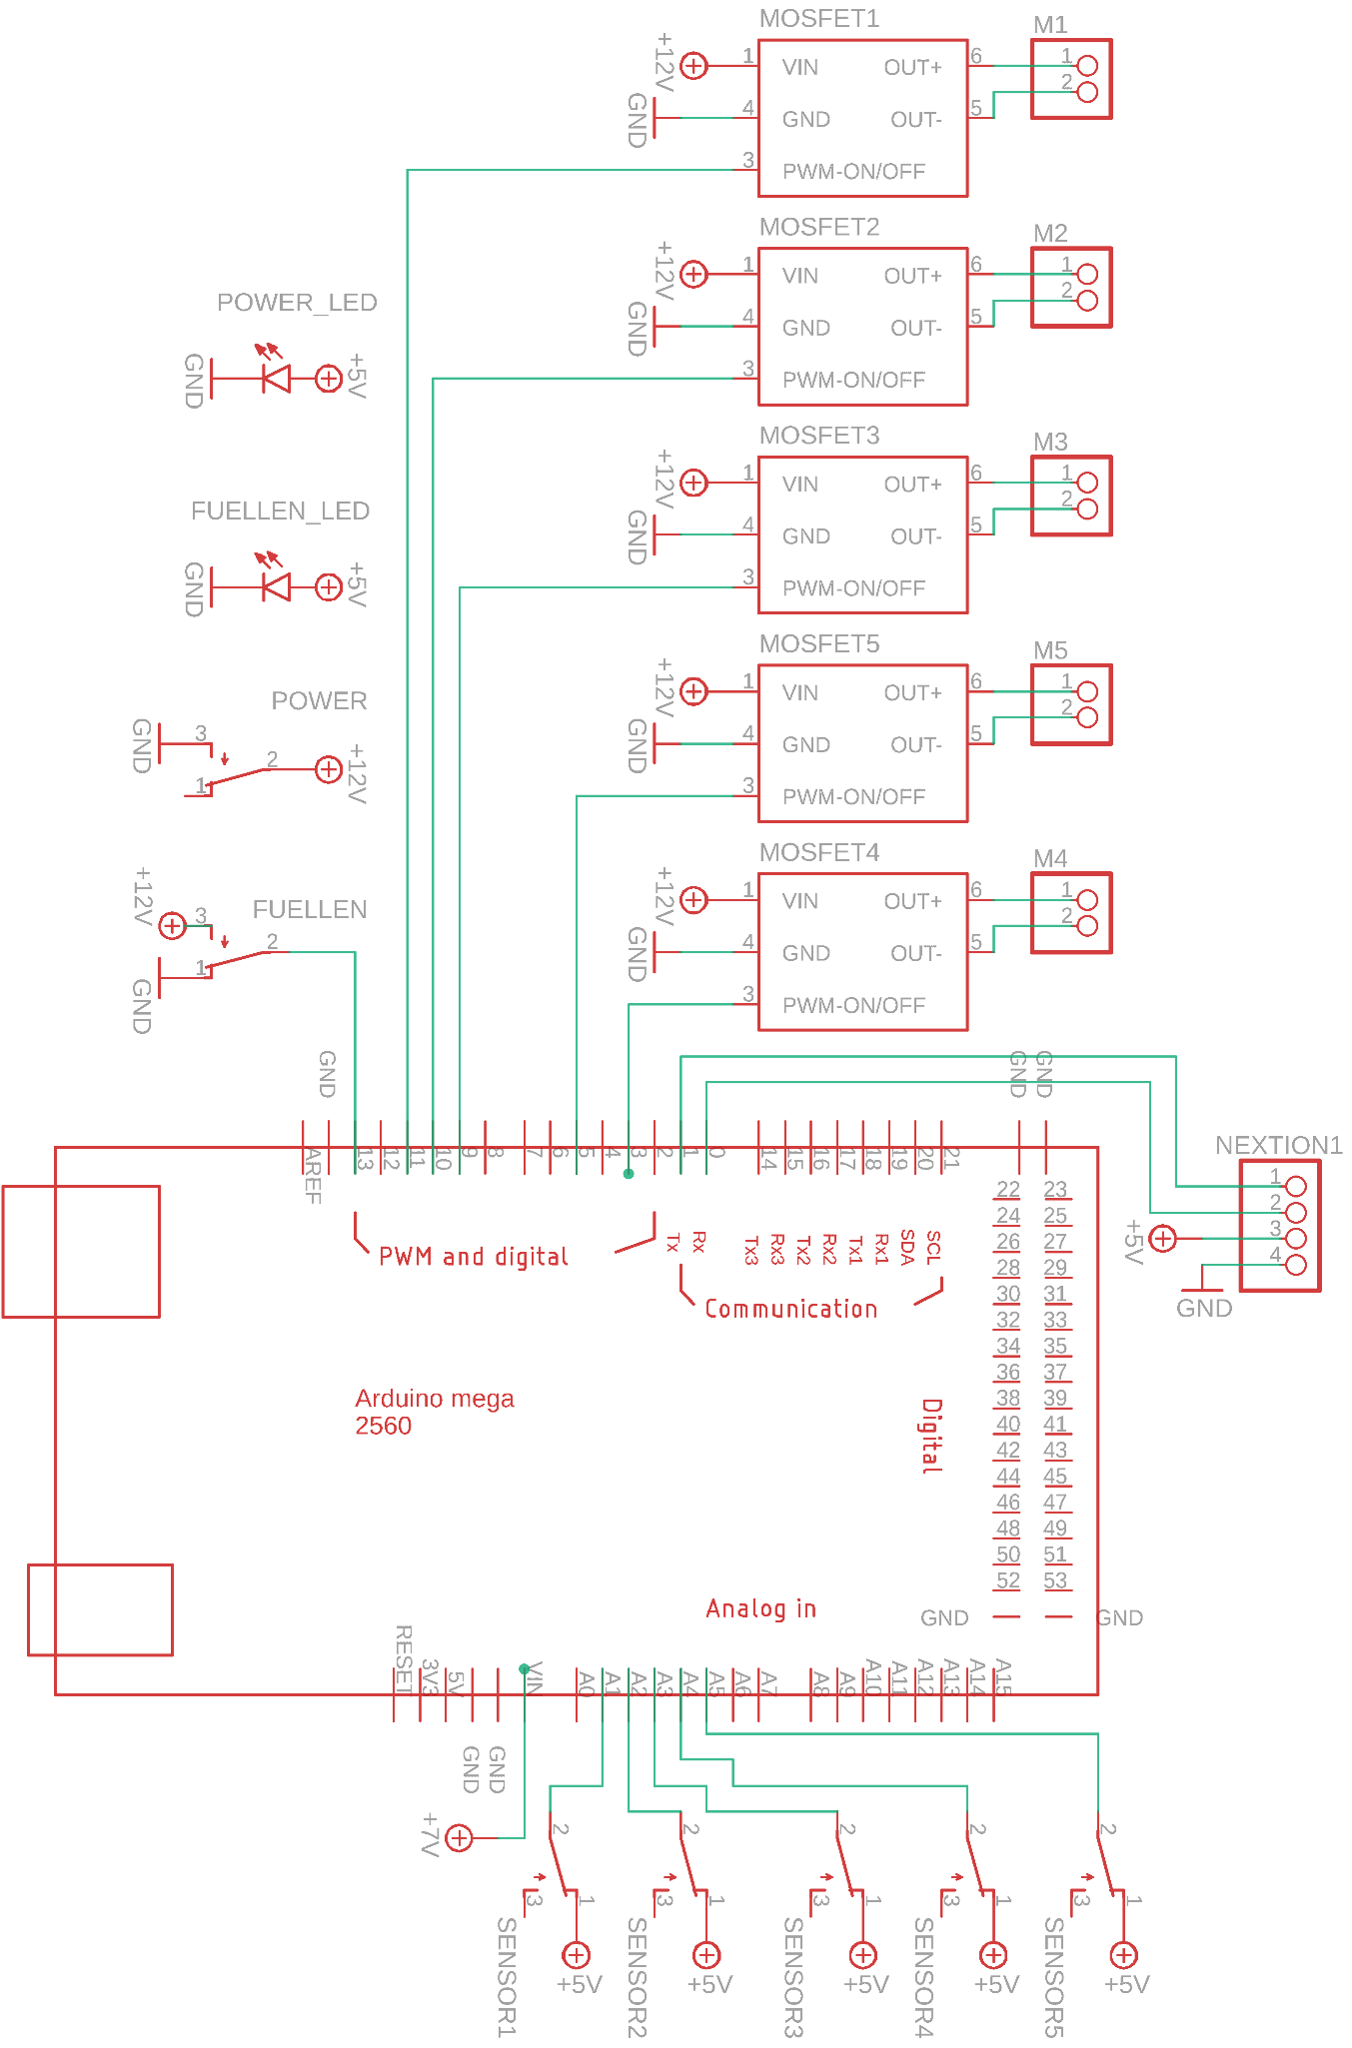
\includegraphics[angle=90, width=\textwidth]{./img/Anhang/Schaltplan.png}}
    \caption{Schaltplan}
\end{figure}

\chapter{Deep Learning Modell für die Klassifizierung}\label{Anhang_E}
\lstinputlisting[language=python, style=algoBericht, basicstyle=\tiny\sffamily, captionpos=b, caption={Deep Learning Modell für die Klassifizierung}, escapeinside={\#*}{*)}]{./Listings/train_dialog_model.py}